\chapter{実験}
\section{実験目的}
シュミレータを用いて実験を行い,提案手法の有効性の検証を行う.
\section{実験環境}
実験はシミュレータ上で行い,
シミュレータ環境としてオープンソースの
3DロボットシミュレータGazebo\cite{gazebo:online}を用いる.
実験装置として,turtlebot3\_waffle\cite{turtlebot3:online}へカメラを
3つ追加したモデルFig. \ref{fig::turtlebot3}を用いる.

\begin{figure}[H]
    \centering
    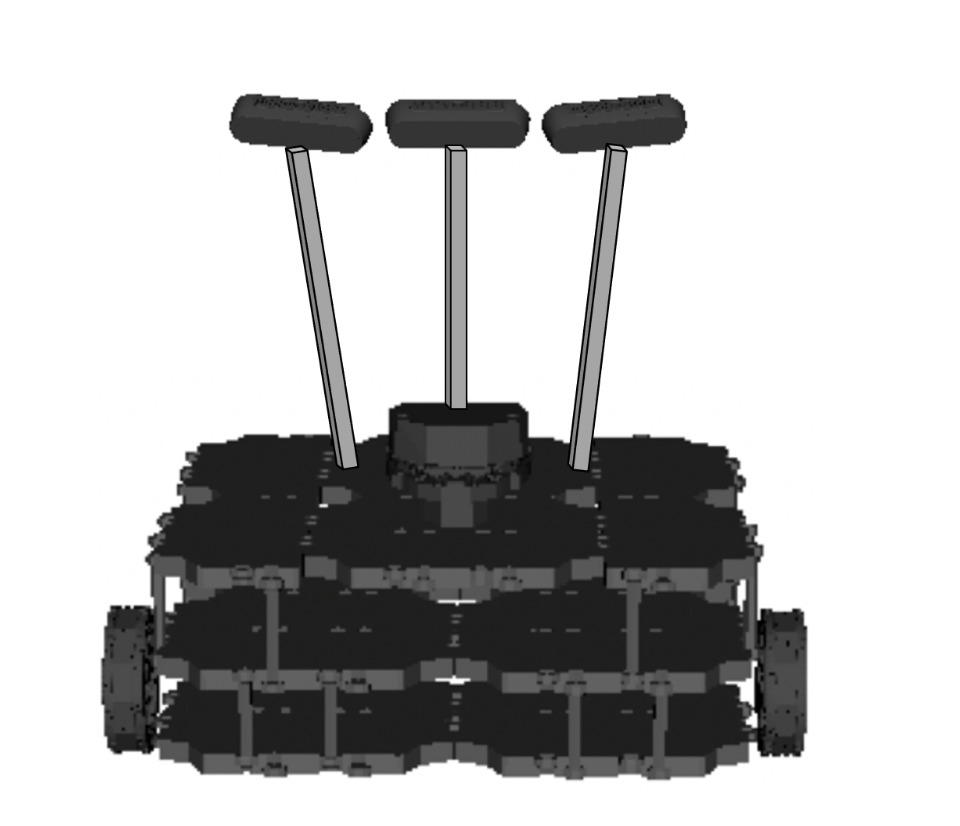
\includegraphics[width = 7cm]{./figs/3_camera.png}
    \caption{Turtlebot3 waffle add 3 cameras}
    \label{fig::turtlebot3}
\end{figure}

\section{実験方法}

実験における手順を下記に示す
\begin{enumerate}
  \item 設定した経路を学習フェーズで走行し,学習器の訓練(経路の学習)行う
  \item テストフェーズへ移行,各経路を設定した回数走行する.
\end{enumerate}
なお,学習器の訓練は「訓練データ (カメラ画像, 目標方向指令) を学習器へ入力し,結果を出力」を 1step とする.
また,データセットの収集及び,学習器への入力は0.25[s]周期で行い,走行に用いる並進速度は0.2[m]とする.

\section{実験条件}
実験条件は
テストフェーズにおいて,
\begin{enumerate}
  \item 成功:壁に衝突せず, 指定した目標地点へ到達
  \item 失敗:目標方向指令とは異なった経路を選択, または壁に衝突
\end{enumerate}
とした.
\newpage
\section{実験1 十字路}
\subsection{実験環境}
Fig. \ref{fig::zyuzi}に環境と経路,入力する目標方向を示す.
環境は2.5m幅の十字路の環境を用いる.
経路は下記の手順を6000[step]学習するまで,繰り返し走行する.
なおB,C,DのTarget pointに到達次第,Startの位置へロボットの位置,姿勢を移動させる.
\begin{enumerate}
  \setlength{\parskip}{0cm} % 段落間
  \setlength{\itemsep}{0cm} % 項目間
  \item Start - A - Target point(B)
  \item Start - A - Target point(C)
  \item Start - A - Target point(D)
  \end{enumerate}

\begin{figure}[ht]
    \centering
    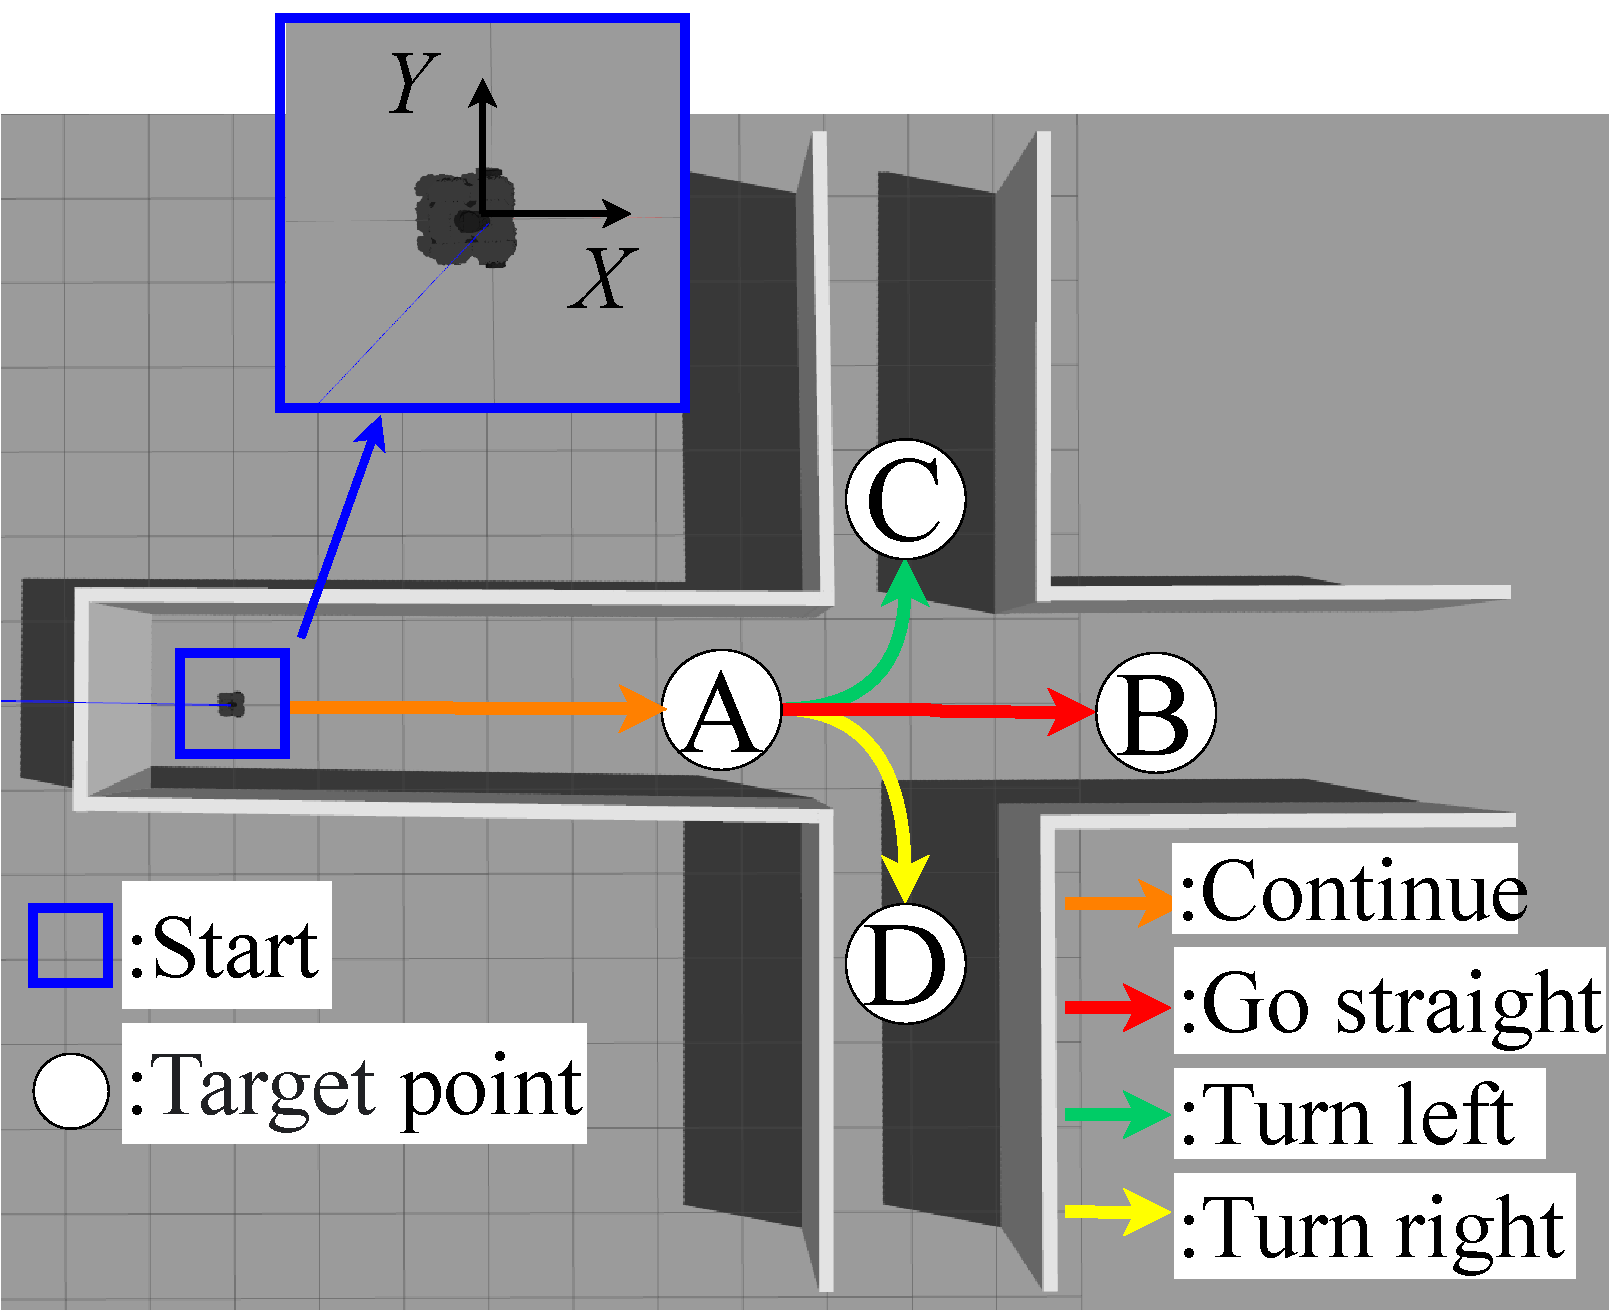
\includegraphics[width = 10cm]{./figs/zyuziroute.pdf}
    \caption{Course of experiment1}
    \label{fig::zyuzi}
\end{figure}

% \newpage
% \subsection{学習フェーズでの経路}
% 学習時の経路についてFig. \ref{fig::exp1route}に示す
% Fig内の緑で示す箇所が初期位置,赤で示す円が目標地点である
% 目標地点を1,2,3の順で走行し,到達後初期値点へロボットの位置,姿勢をリセットする.

% \begin{figure}[ht]
%     \centering
%     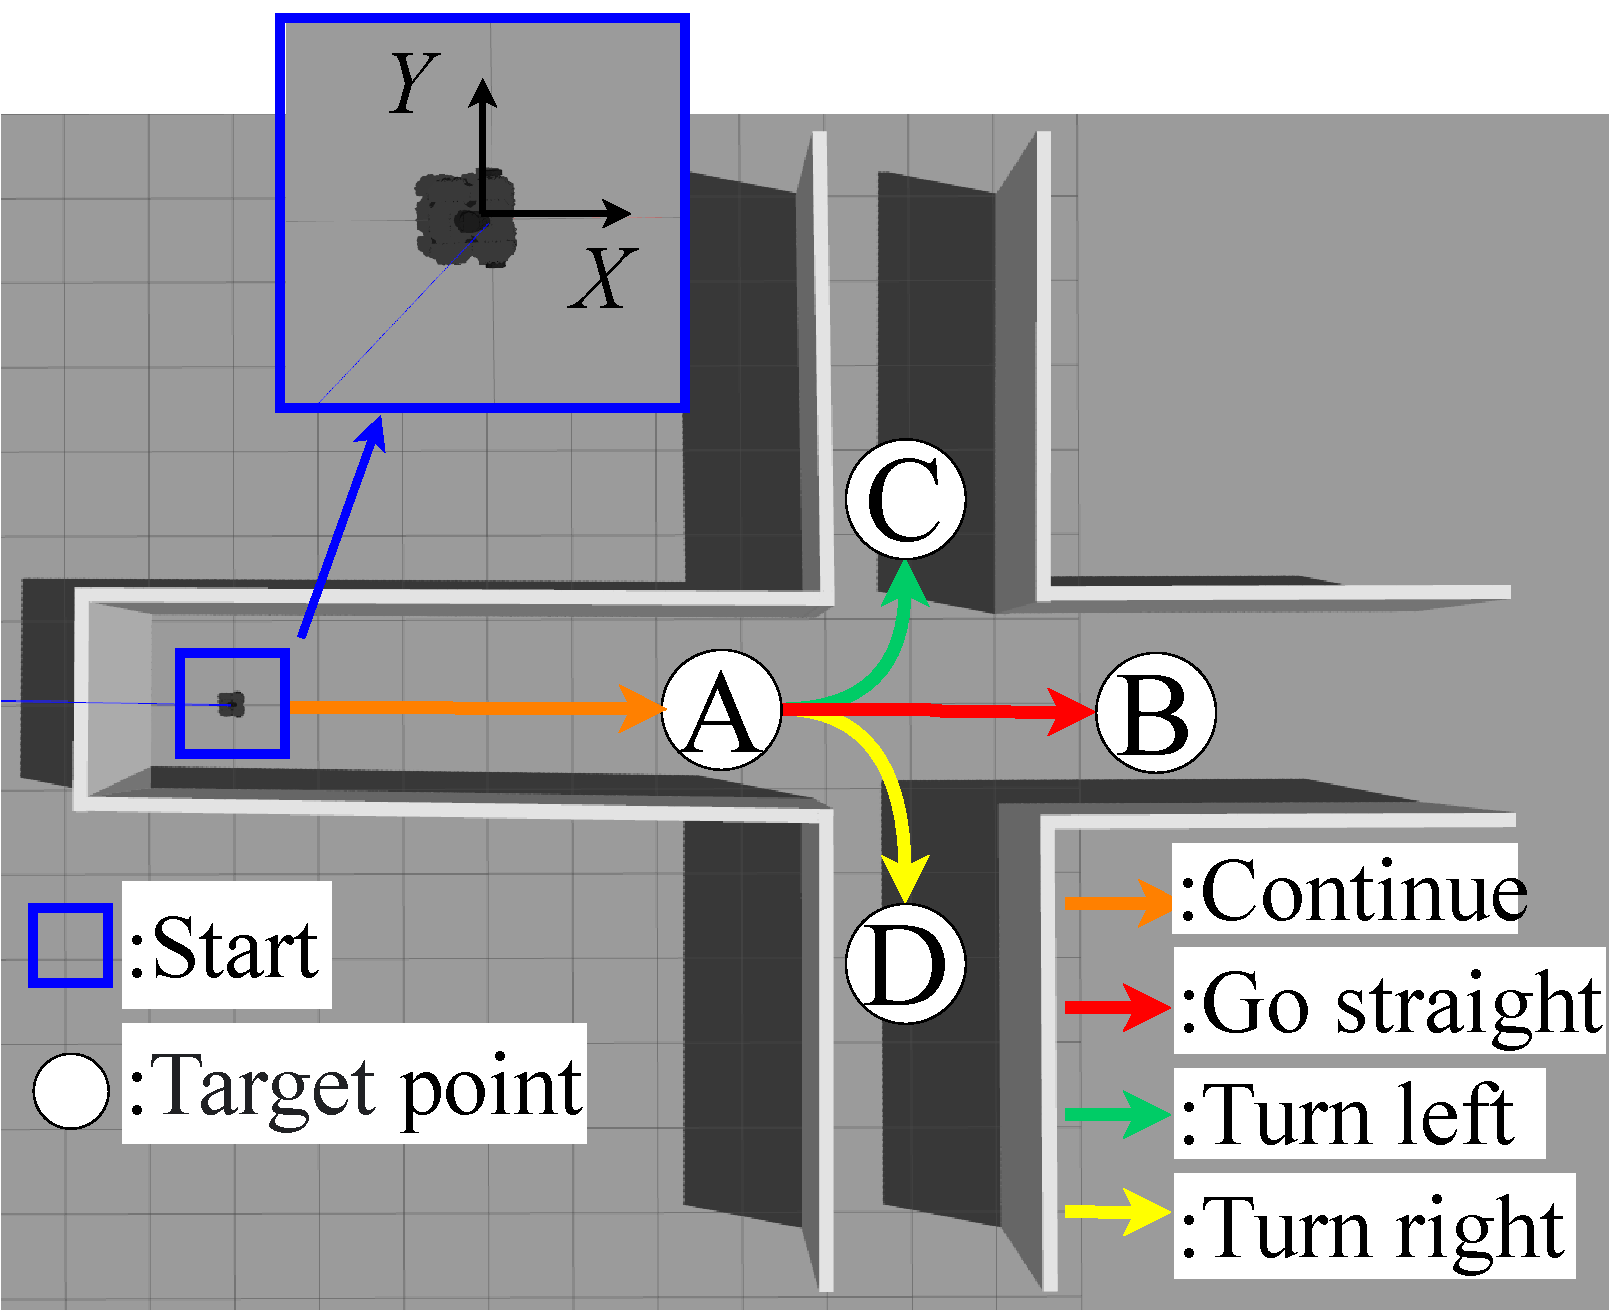
\includegraphics[width = 10cm]{./figs/zyuziroute.pdf}
%     \caption{Route of experiment 1}
%     \label{fig::exp1route}
% \end{figure}

\subsection{評価}
% Fig. \ref{fig::exp1route}で青で示した地点において,
% コマンドを入力を行った結果をTable. \ref{tb::exp1suc}に示す.
テストフェーズで,各経路を10回ずつ走行した結果を表\ref{tb::exp1suc}に示す.
すべての経路において,目標地点へ到達することに成功した
% \begin{table}[H]
%   \centering
%   \caption{Number of successes experiment 1 point}
%   \begin{tabular}{|c|c|}
%   \hline
%   Point & Number of successes \\ \hline
%   1     & 5/5                  \\ \hline
%   2     & 4/5                  \\ \hline
%   3     & 5/5                  \\ \hline
%   \end{tabular}
  
%   \label{tb::exp1suc}
%   \end{table}
\begin{table}[h]
  \caption{Number of successes experiment}
  \label{tb::exp1suc}
  \begin{center}
      \vskip 0.5zh
      \begin{tabular}{|c|c|}
          \hline
          Route & Number of successes\\ \hline
          % Start - A (continue) & $10/10$ \\ \hline
          Start - A - B  & $10/10$ \\ \hline
          Start - A - C  & $10/10$ \\ \hline
          Start - A - D  & $10/10$ \\ \hline
      \end{tabular}
  \end{center}
\end{table}


\newpage
\section{実験2 -8の字-}
% \subsection{実験目的}
% 実験1で用いた局所的な環境を更に複雑な環境へ拡張し,
% 提案手法を用いて,分岐路においてコマンドによってルートの変更が可能であるかさらなる検証を行う.
\subsection{実験環境}
Fig. \ref{fig::hatinozi}に示した,縦8[m]×横12[m]で道幅が2.5[m]の8の字型の環境を用いる
\begin{figure}[h]
    \centering
    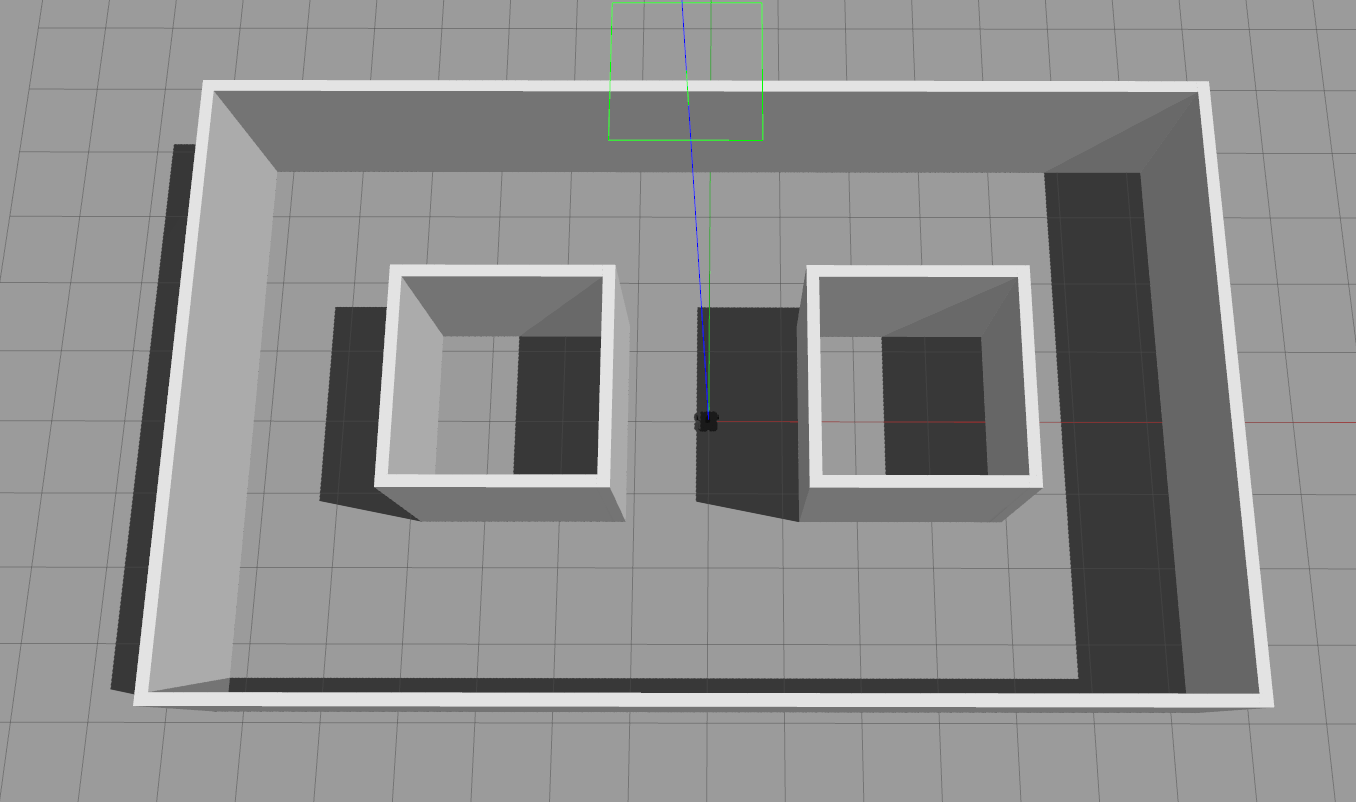
\includegraphics[width = 10cm]{./figs/coli.png}
    \caption{Experiment2 Course}
    \label{fig::hatinozi}
\end{figure}

\newpage
\ref{fig::exp2route}に示す環境内を網羅する経路をRoute A-Fの順で60000[step]学習するまで,繰り返し走行する.
\begin{figure}[H]
    \begin{tabular}{cc}
      \begin{minipage}[t]{0.5\hsize}
        \centering
        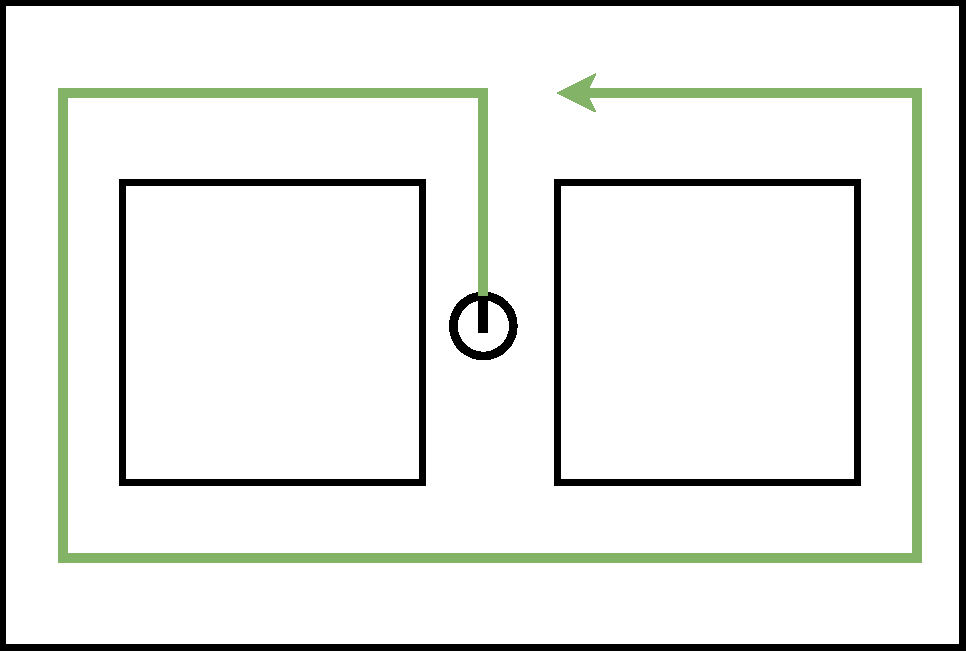
\includegraphics[keepaspectratio, scale=0.4]{./figs/8nozi_1.pdf}
        \subcaption{Route A}
        \label{exp2route1}
      \end{minipage} 
      \begin{minipage}[t]{0.5\hsize}
        \centering
        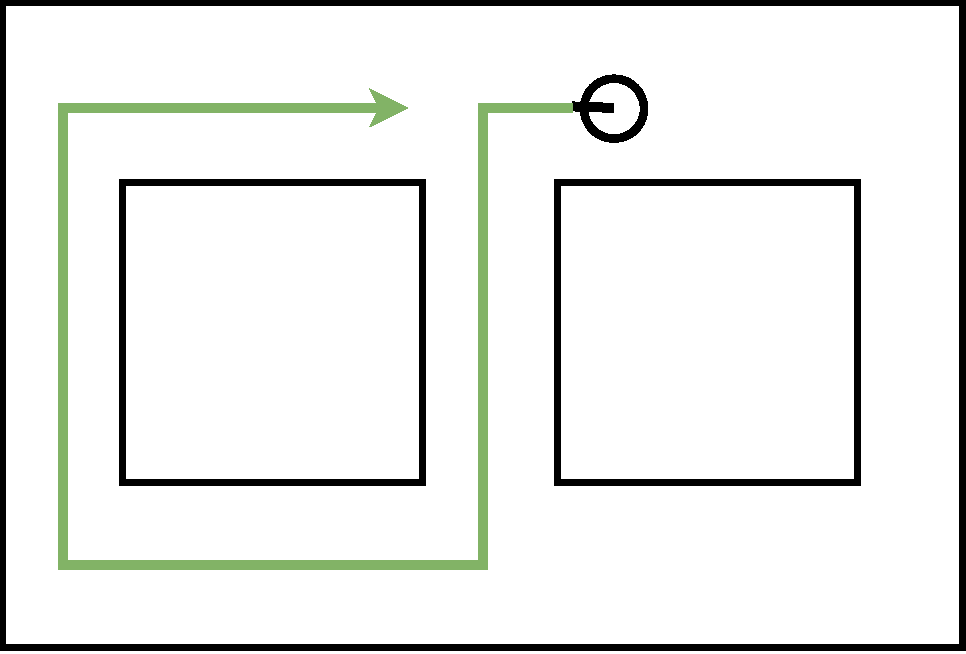
\includegraphics[keepaspectratio, scale=0.4]{./figs/8nozi_2.pdf}
        \subcaption{Route B}
        \label{exp2route2}
      \end{minipage} \\
      \vspace{2.0zh}
      \begin{minipage}[t]{0.5\hsize}
        \centering
        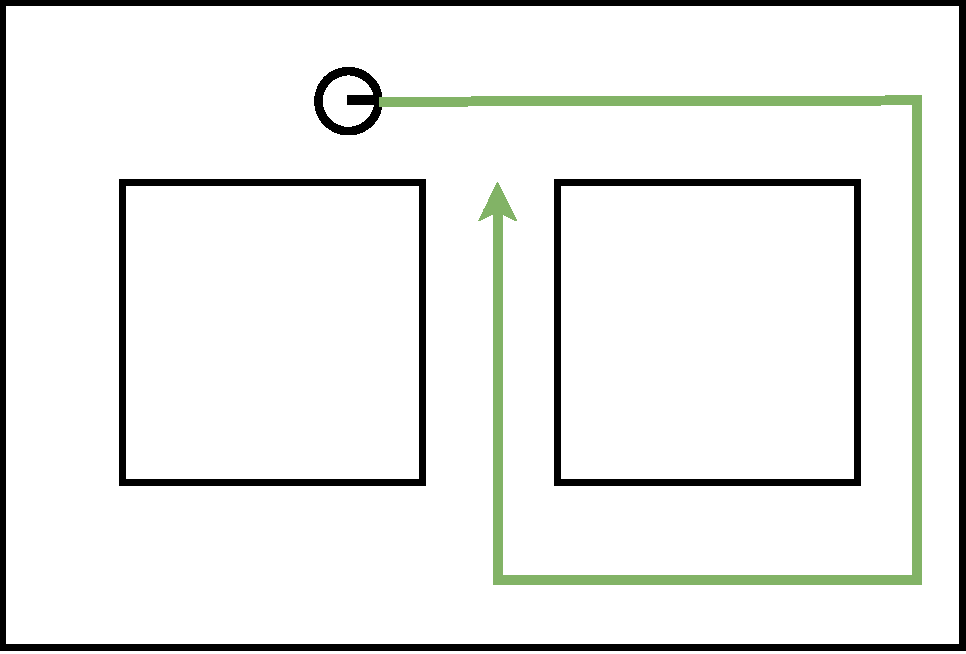
\includegraphics[keepaspectratio, scale=0.4]{./figs/8nozi_3.pdf}
        \subcaption{Route C}
        \label{exp2route3}
      \end{minipage} 
      \begin{minipage}[t]{0.5\hsize}
        \centering
        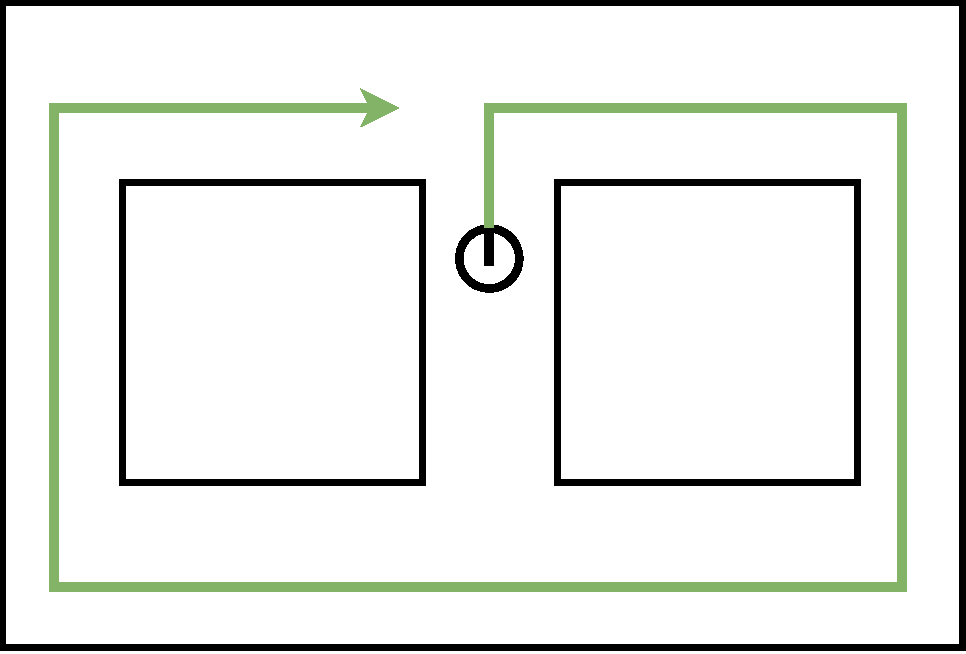
\includegraphics[keepaspectratio, scale=0.4]{./figs/8nozi_4.pdf}
        \subcaption{Route D}
        \label{exp2route4}
      \end{minipage}\\

      \begin{minipage}[t]{0.5\hsize}
        \centering
        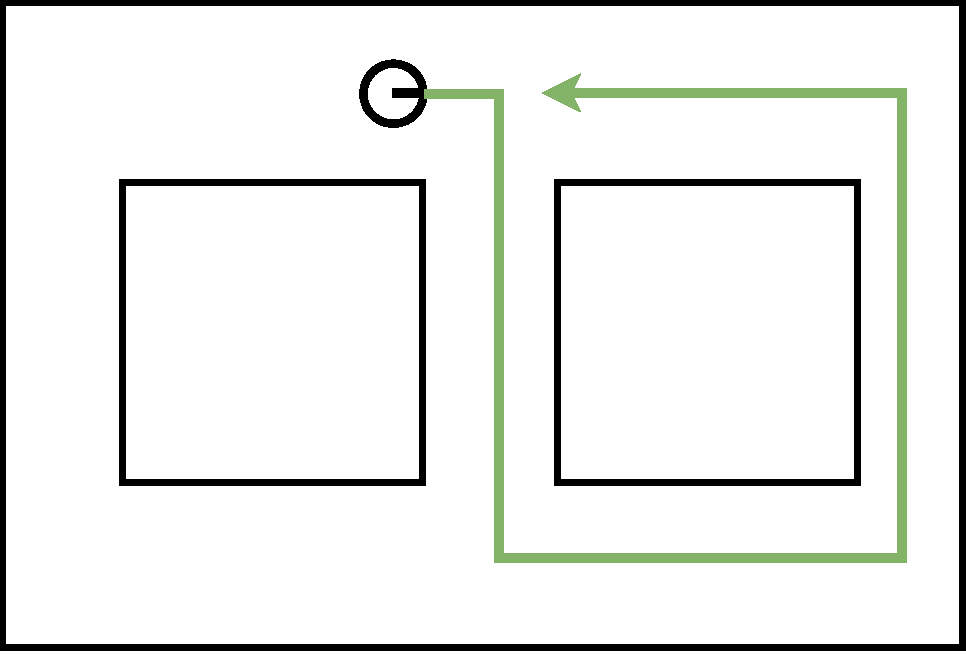
\includegraphics[keepaspectratio, scale=0.4]{./figs/8nozi_5.pdf}
        \subcaption{Route E}
        \label{exp2route5}
      \end{minipage} 
      \begin{minipage}[t]{0.5\hsize}
        \centering
        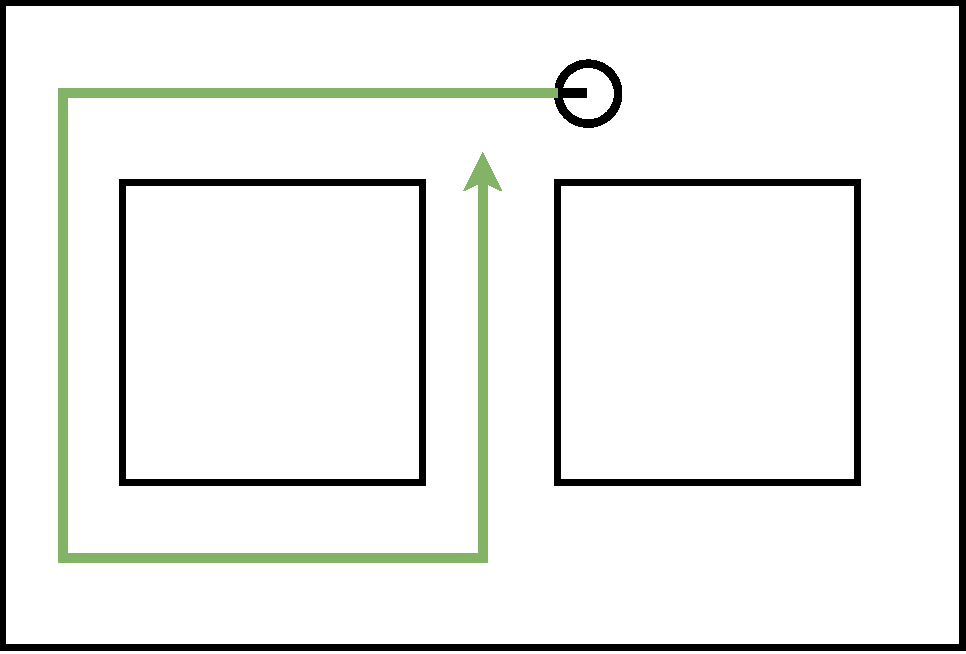
\includegraphics[keepaspectratio, scale=0.4]{./figs/8nozi_6.pdf}
        \subcaption{Route F}
        \label{exp2route6}
      \end{minipage} 
    \end{tabular}
     \caption{Experiment 2 route}
     \label{fig::exp2route}
  \end{figure}
  
\newpage
\subsection{評価}
テストフェーズで,経路をランダムに60回走行を行った結果をTable. \ref{tb::exp2suc}に示す.
% % \begin{figure}[h]
% %   \centering
% %   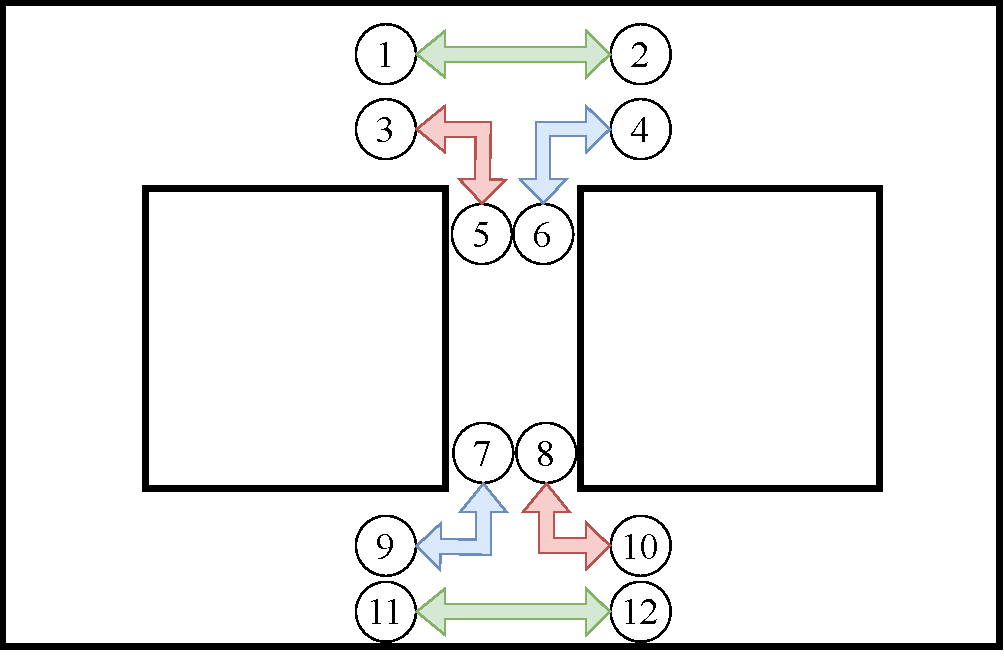
\includegraphics[width = 10cm]{./figs/bunkiban.pdf}
% %   \caption{Experiment 2 point number}
% %   \label{fig::bunkiban}
% % \end{figure}

% \begin{table}[H]
%   \centering
%   \caption{Number of successes Experiment2 point}
%   \begin{tabular}{|c|c|}
%   \hline
%   Route & Number of successes \\ \hline
%   A     & 10/10                  \\ \hline
%   B     & 10/10                  \\ \hline
%   C     & 10/10                  \\ \hline
%   D     & 0/10                  \\ \hline
%   E     & 10/10                  \\ \hline
%   F     & 10/10                  \\ \hline
%   \end{tabular}
%   \label{tb::exp2suc}
%   \end{table}
%   \subsection{評価}
  
  \begin{table}[htb]
    \centering
    \caption{Number of successes Experiment2 point}
    \begin{tabular}{|c|c|}
    \hline
    Route & Number of successes \\ \hline
    A-F     & 50/60                  \\ \hline
    \end{tabular}
    \label{tb::exp2suc}
    \end{table} 